%
% ─── PLANIFICACION Y PRESUPUESTO ────────────────────────────────────────────────
%

Hasta el momento hemos introducido la materia matemática básica de esta disciplina y las herramientas gráficas utilizadas en informática gráfica. Con el objetivo de familiarizar al usuario de internet con los conjuntos de Julia y Mandelbrot en dos dimensiones, estudiados en el capítulo \ref{chap:Julia-Mandelbrot}, y con el de conseguir nuestras primeras visualizaciones de fractales tridimensionales es momento de comenzar el desarrollo del producto software. Como se ha dicho en la introducción y en otras partes de esta memoria, este producto consiste en una web interactiva en la que poder graficar distintos fractales, tanto 2D como 3D, permitiendo modificar algunos de sus parámetros de manera dinámica.  

\section{Planificación}

A continuación describiremos la planificación temporal por fases de este producto software. Debe tenerse en cuenta que con cada avance hay asociado un tiempo de codificación de la funcionalidad, pero también un tiempo buscando información, consultando bibliografía y redactando la documentación del software.

\subsection{Infraestructura básica}

La fase de desarrollo comienza a principios de Febrero de 2022, digamos el día 8. El primer paso es conseguir una web vacía con un elemento tipo `canvas' en el cual visualicemos algo sencillo, como por ejemplo un cuadrado de colores.

Esta tarea es sencilla, ya que hay muchos tutoriales, es el `hello world' de las aplicaciones gráficas. Debe estar lista antes del día \textbf{11 de Febrero de 2022}.

Con esto, ya tenemos la infraestructura básica del producto software.

\subsection{Visualización de fractales 2D}

Con el código hasta ahora, debemos modificar la estructura para que el software grafique los primeros fractales 2D de forma estática. Primero bastará con graficarlos en blanco y negro para posteriormente añadir colores.

Seguidamente, debemos preparar el documento web para el soporte de interactividad y gestión de eventos. Es decir, añadir formularios, botones, deslizadores... en principio sin funcionalidad alguna. Hecho esto, añadimos definitivamente la interactividad, permitiendo que a partir del documento web se pueda interactuar con el canvas y la escena que se está visualizando. Con cada avance en el desarrollo debe cuidarse la apariencia y el estilo de la web.

En este punto, el producto consiste en una web interactiva para visualizar fractales en 2D. Esta tarea no es tampoco demasiado compleja al ser sencillo identificar un canvas 2D con una región del plano sencilla, pero requiere mucha funcionalidad muy distinta, la cual es la primera vez que se programa, y teniendo en cuenta que es una parte importante del proyecto que servirá de base para el resto de fases, estipulamos que debemos dar como margen hasta el \textbf{25 de Marzo de 2022}.

\subsection{Construcción de un programa ray-tracer}

Comenzando con la parte tridimensional del software, aprovechamos gran parte del código ya desarrollado para la escena 2D, pues realmente el documento web puede tener la misma forma y la interacción con sus elementos es similar, aunque adaptada a los distintos parámetros que admite una escena 3D como son la posición o la iluminación.

El primer paso para tener una web en la que visualizar una escena con fractales es empezar graficando cuerpos sencillos utilizando ray-tracing. Por tanto, lo primero que haremos será un pequeño programa que mediante ray-tracing visualice una escena sencilla con esferas y un plano (a modo de suelo) que nos permita movernos libremente por el espacio. Aplicaremos también un modelo de iluminación local sencillo para aportar un poco de realismo a la escena.

A la par, debemos seguir cuidando tanto el estilo del documento web como la posibilidad de interactuar con la página. Por suerte, a partir del código ya desarrollado en la anterior fase, esta tarea se facilita considerablemente respecto a las primeras veces.

Este programa requiere programar el propio ray-tracing, formas de calcular las intersecciones de los rayos con los objetos, llenar de objetos la escena, parametrizar la posición de la cámara e implementar el modelo de iluminación. La tarea es generalmente compleja, pero está muy basada en el código ya implementado para fractales 2D, por lo que estimamos que debe estar programada para el día \textbf{22 de Abril de 2022}.

\subsection{Visualización de fractales en 3D}

Esta aunque no es la última fase del desarrollo del producto, probablemente sí sea la más importante y la más compleja. Debemos modificar el programa ray-tracer del apartado anterior con el objetivo de visualizar en la escena imágenes de fractales 3D.

Esta fase requiere, además de código, mucho tiempo de búsqueda y consulta bibliográfica. Una vez adquiridos conocimientos necesarios haremos las modificaciones oportunas a las regiones de código necesarias al programa que tenemos hasta ahora con el objetivo de visualizar los fractales en 3D.
Al igual que en todas las fases, debemos ir añadiendo parámetros modificables a la web y cuidar el estilo.

Una vez realizado esto, contaríamos con una web en la que interactuar con fractales 2D o 3D, pudiendo visualizar de forma concreta y sencilla estas singulares figuras. Esto finalizaría la parte más compleja y también la más necesaria del proyecto, pues es la que cumple el objetivo fundamental. Estipulamos por tanto que debe estar lista alrededor del día \textbf{13 de Mayo de 2022}.

\subsection{Realismo y optimización en la escena 3D}

Aunque la funcionalidad está completa y el objetivo cumplido, es bueno pulir algunos detalles relacionados con el realismo. Por ejemplo, añadir la visualización de sombras arrojadas al modelo de iluminación o técnicas como el antialiasing para suavizar los bordes.

El problema es que estas dos adiciones son muy costosas en tiempo, lo cual compromete la velocidad de ejecución, por lo que añadiremos a la web la posibilidad de elegir si se desean aplicar o no.

Seguidamente podemos añadir esferas englobantes al programa como técnica de optimización, al menos en escenas donde el fractal esté relativamente lejano.

Estas modificaciones completarían el desarrollo software de la visualización e interacción de la escena y en lo que a `backend' se refiere completa el software. Debe estar lista el \textbf{1 de Junio de 2022}.

\subsection{Añadir estilo y UX a la web}

Desde el inicio, al estar en fases de desarrollo, hemos descuidado bastante la apariencia de la página en lo que a secciones, fuentes y colores se refiere. Por tanto, añadiremos estilo y código CSS al documento para darle una apariencia más visual y amigable.

La última, pero no por ello menos importante fase del desarrollo debe estar finalizada el día de la entrega, que es el \textbf{20 de Junio de 2022}.

\vspace{0.5cm}

En conclusión, y a modo de resumen, presentamos en la imagen \ref{fig:Gantt} el conocido como \textit{diagrama de Gantt}, que sintetiza en una tabla el tiempo dedicado a cada actividad. Cada columna representa una semana, identificada por el día y el mes del lunes de dicha semana.

\begin{figure} [ht]
    \centering
    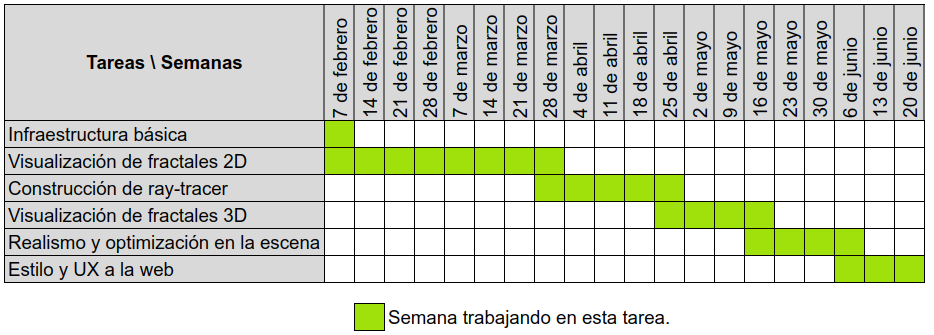
\includegraphics[scale = 0.44]{img/Gantt.png}
    \caption{Diagrama de Gantt de la planificación del desarrollo del producto software}
    \label{fig:Gantt}
\end{figure}


\section{Presupuesto del producto software}

A continuación haremos una estimación del presupuesto de este producto. Para ello desglosaremos los distintos recursos utilizados en: recursos hardware, recursos software y recursos humanos. Estimaremos el coste de cada uno de ellos y presentaremos un presupuesto final.

\subsection{Recursos hardware}

Todo el software ha sido desarrollado en un ordenador portátil personal. Las especificaciones hardware de dicho ordenador se pueden comprobar en la tabla \ref{tabla:especificaciones-PC}.
\begin{table}[ht]
    \centering
    \begin{tabular}{ll}
    \hline
    Modelo                           & HP Pavilion 15 Notebook PC                       \\ \hline
    Procesador                       & Intel Core i7-4500U                              \\ \hline
    \multirow{2}{*}{GPU} & nVidia GeForce 840M                              \\
                                     & Intel Haswell-ULT Integrated Graphics Controller \\ \hline
    RAM                              & 7.7 GiB                                          \\ \hline
    Sistema Operativo                & Ubuntu 20.04.2 LTS                               \\ \hline
    \end{tabular}
    \caption{Especificaciones del PC en el que se ha desarrollado el proyecto}
    \label{tabla:especificaciones-PC}
    \end{table}


El ordenador fue estrenado el 6 de enero de 2016, fue adquirido por un precio de 620€. Este enero ha cumplido seis años de uso, por lo que su valor es mucho menor. Estimando el rendimiento que suele ofrecer y el estado de sus componentes hardware en general, se estima que a día de hoy costaría unos \textbf{70€}.

\subsection{Recursos Software}

A continuación enumeraremos los recursos software utilizados en la codificación y en la documentación.

\begin{itemize}
    \item \textbf{Visual Studio Code}: Editor de código utilizado tanto para redactar todo el código fuente necesario como la memoria, gracias a sus múltiples extensiones que lo convierten en un entorno de desarrollo muy versátil.
    \item \textbf{Google Chrome}: Navegador web, ampliamente utilizado para visualizar la web que se ha desarrollado en cada una de sus fases. también se ha empleado para consultar bibliografía, buscar información o realizar muchas de las imágenes utilizadas. En este último aspecto, los sitios más visitados han sido \href{https://www.vectary.com/}{\textcolor{blue}{Vectary}} y  \href{https://www.figma.com/}{\textcolor{blue}{Figma}}.
    \item \textbf{Git y Github}: Sistema de control de versiones, gracias a git se ha permitido llevar un histórico de los avances que se han hecho en el trabajo. Además, con `github' pages se ha podido desplegar la web en internet gratuitamente.
    \item \textbf{Bootstrap}: Framework de CSS y JavaScript útil para la programación del estilo de la página web.
    \item \textbf{jQuery}: Biblioteca de JavaScript que simplifica la sintaxis y la programación del lenguaje.
\end{itemize}

Todo esto junto con las típicas aplicaciones como el navegador de archivos, la terminal, etc.

Afortunadamente, todos los recursos software son gratuitos, por lo que el presupuesto de los recursos software se reduce a \textbf{0€}.

\subsection{Recursos humanos}

Sobre recursos humanos, el producto ha sido en su totalidad desarrollado por el alumno y autor de este texto: Juan Antonio Villegas Recio. Siempre bajo la supervisión y ayuda del tutor de informática: D. Carlos Ureña Almagro.

Si hacemos una estimación de unas 20 horas semanales de media, teniendo en cuenta que el desarrollo ha durado 20 semanas, lo cual supone un total de 400 horas, a régimen de 15€ por cada hora de trabajo, en total el gasto en recursos humanos supone \textbf{6.000€}.

\subsection{Presupuesto final}

Presentamos entonces el desglose final del presupuesto de este proyecto en la tabla \ref{tab:presupuestos}.

\begin{table}[ht]
    \centering
    \begin{tabular}{ll}
    \hline
    \textbf{Recurso}     & \textbf{Precio} \\ \hline
    Recursos hardware    & 70€             \\ \hline
    Recursos Software    & 0€              \\ \hline
    Recursos humanos     & 6000€           \\ \hline
    \textbf{Coste total} & \textbf{6070€}  \\ \hline
    \end{tabular}
    \caption{Desglose por recursos del presupuesto final}
    \label{tab:presupuestos}
\end{table}

Por tanto, el presupuesto de este producto software es de \textbf{6070€}.

\section{Análisis de requisitos}

Una vez estimada la planificación temporal y el presupuesto del proyecto, es momento de definir correctamente los requisitos y la funcionalidad que ofrecerá el producto. Para ello, haremos un análisis de requisitos del problema, estableceremos sus casos de uso y veremos mediante un diagrama las interacciones entre los mismos.

Tras un estudio profundo del problema y evaluando la viabilidad de los mismos, introducimos los requisitos, funcionales y no funcionales, de este producto:

\subsection{Requisitos funcionales}
En caso de la visualización de fractales 2D:
\begin{itemize}
    \item \textbf{RF1.1}: Visualización de conjuntos de Julia y Mandelbrot 2D.
    \item \textbf{RF1.2}: Posibilidad de alternar qué fractal ver en el canvas: Julia o Mandelbrot.
    \item \textbf{RF1.3}: Posibilidad de cambiar el exponente $m$ de la función $P_{c,m}(z)=z^m+c$ para poder visualizar conjuntos de Julia y Mandelbrot generalizados.
    \item \textbf{RF1.4}: Posibilidad de cambiar la constante $c$ de la función $P_{c,m}(z)=z^m+c$ en el caso de los conjuntos de Julia para poder visualizar diferentes conjuntos de Julia $\mathcal{J}_c$ para distintos $c\in\C$.
    \item \textbf{RF1.5}: Poder movernos libremente por el plano.
    \item \textbf{RF1.6}: Hacer zoom de forma que podamos observar las infinitas irregularidades que presentan los fractales.
    \item \textbf{RF1.7}: Modificar los parámetros que acepten los algoritmos utilizados para visualizar los fractales para ver cómo cambia la imagen al cambiar dichos parámetros.
\end{itemize}
En caso de fractales 3D:
\begin{itemize}
    \item \textbf{RF2.1}: Visualización de generalizaciones tridimensionales de los conjuntos de Julia y Mandelbrot.
    \item \textbf{RF2.2}: Posibilidad de alternar qué fractal 3D ver en el canvas en cada momento.
    \item \textbf{RF2.3}: Posibilidad de modificar parámetros del modelo de iluminación para así observar distintos materiales y coloraciones en los fractales.
    \item \textbf{RF2.4}: Modificar parámetros de los algoritmos de visualización que empleemos.
    \item \textbf{RF2.5}: Posibilidad de moverse libremente por la escena utilizando una cámara orbital.
    \item \textbf{RF2.6}: Hacer zoom en la escena para poder observar de cerca las superficies de los fractales.
\end{itemize}
De forma genérica:
\begin{itemize}
    \item \textbf{RF3}: Botón de reseteo para restablecer los valores de los parámetros por defecto.
    \item \textbf{RF4}: Posibilidad de cambiar rápidamente entre visualización 2D y 3D.
\end{itemize}

\subsection{Requisitos no funcionales}

\begin{itemize}
    \item \textbf{RNF1}: El tiempo de procesado no debe ser demasiado largo. A ser posible se ejecutará en tiempo real.
    \item \textbf{RNF2}: Deben utilizarse herramientas portables, es decir, que puedan ejecutarse en cualquier navegador sin necesidad de instalar nada.
    \item \textbf{RNF3}: La interfaz de usuario tiene que ser sencilla, para que pueda utilizarla cualquier persona.
    \item \textbf{RNF4}: El software debe poder ser ejecutado en cualquier ordenador estándar. Por tanto, las técnicas utilizadas no pueden requerir un hardware demasiado avanzado ni demasiado caro.
    \item \textbf{RNF5}: Es necesario incluir cierta documentación en la web para que el usuario con pocos conocimientos sepa identificar el uso de cada parámetro.
    \item \textbf{RNF6}: Deben usarse colores e interfaces que cuiden la experiencia de usuario.
    \item \textbf{RNF7}: No será posible elegir valores de parámetros imposibles o que requieran una cantidad inviable de cálculo.
\end{itemize}

\subsection{Requisitos de datos}

No existen requisitos de datos, ya que no hay realmente ninguna base de datos ni es necesaria, pues no es una aplicación que almacene datos, sino que realiza cálculos para graficar imágenes.

\section{Análisis de casos de uso}

A continuación describiremos los posibles casos de uso del software a desarrollar:
\begin{itemize}
    \item \textbf{CU1}: Primer acceso a la página. El usuario accede por primera vez a la página.
    \item \textbf{CU2}: Modificar un parámetro. El usuario cambia uno de los distintos parámetros modificables.
    \item \textbf{CU3}: Comprobar si un nuevo parámetro es incorrecto o inviable. Ante el cambio de un parámetro, es necesario comprobar que no se ha introducido un valor imposible o computacionalmente inviable. Por ejemplo, un número negativo o demasiado grande de iteraciones.
    \item \textbf{CU4}: Web sobrecargada. Posible sobrecarga provocada por una excesiva demanda de cálculo en poco tiempo.
    \item \textbf{CU5}: Establecer valores por defecto. Cambiar los parámetros de la escena a los que se toman por defecto.
    \item \textbf{CU6}: Dibujar la escena. Visualizar la escena a partir de los parámetros actuales, estando seguros de que son correctos.
    \item \textbf{CU7}: Mensaje de error. Ante cualquier error posible, se notifica del mismo al usuario.
\end{itemize}

Ante estos casos de uso, en la figura \ref{fig:casos-uso} vemos el diagrama de casos de uso, en el cual vemos a cuales de ellos puede acceder el usuario y qué interdependencias hay entre los mismos.

\begin{figure} [ht]
\centering
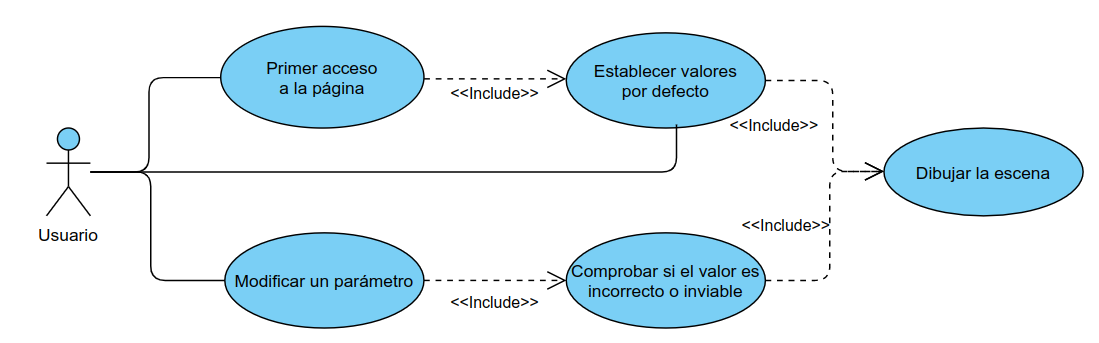
\includegraphics[scale = 0.6]{img/diagrama-CU.png}
\caption{Diagrama de Casos de Uso}
    \label{fig:casos-uso}
\end{figure}

\newpage
\section{Bocetos de la web}

A continuación presentaremos los bocetos básicos, a veces llamados `wireframes', de la apariencia que tendrá la web. Son únicamente tres pantallas, y dos de ellas son prácticamente iguales en lo que a nivel de boceto se refiere. La pantalla en la que se visualizan fractales 2D y 3D en un canvas (imagen \ref{fig:wireframe-fractals}) es prácticamente igual en ambos casos, por lo que sólo hemos incluido una de ellas entendiendo que los enlaces y los títulos son intercambiables en cada versión. 

\begin{figure} [ht]
    \centering
    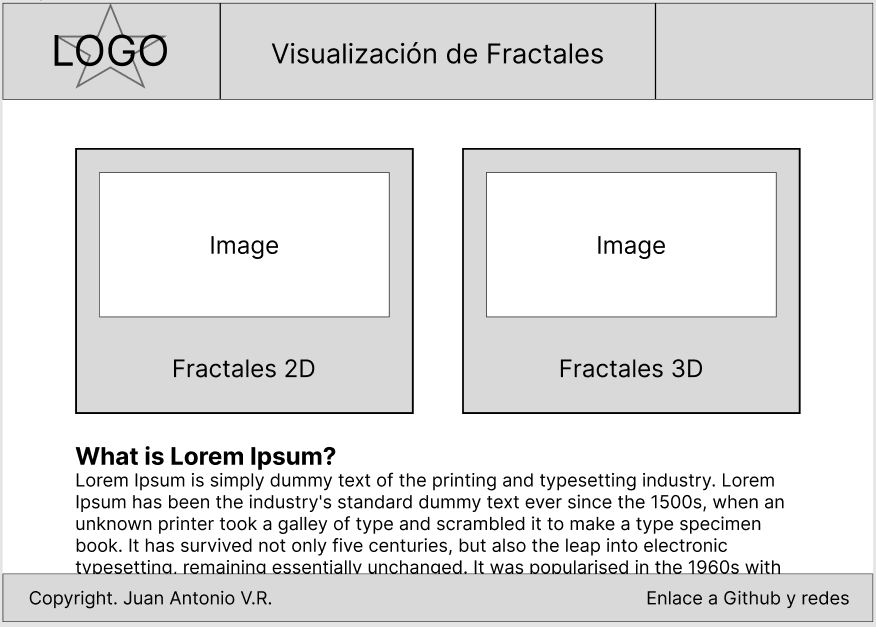
\includegraphics[width=12cm]{img/wireframe-home.png}
    \caption{Wireframe de la portada de la página}
    \label{fig:wireframe-home}
    \end{figure}



Como vemos en la imagen \ref{fig:wireframe-home}, al acceder a la web nos aparecería la posibilidad de elegir si queremos explorar el mundo de los fractales 2D o 3D. Debajo del menú seleccionable aparecería una breve introducción al mundo de los fractales desde un punto de vista entendible por casi cualquier persona con conocimientos básicos.


\newpage

Sobre la pantalla de la imagen \ref{fig:wireframe-fractals}, aparecería a la izquierda el canvas donde se visualizarían los fractales y los distintos controles y parámetros modificables estarían en el lado derecho. Debajo de esta sección de la pantalla también se incluiría un texto documentando el sentido de cada parámetro para que el usuario que no conozca demasiado el trasfondo matemático ni informático pueda interactuar sin problemas.

\begin{figure} [ht]
    \centering
    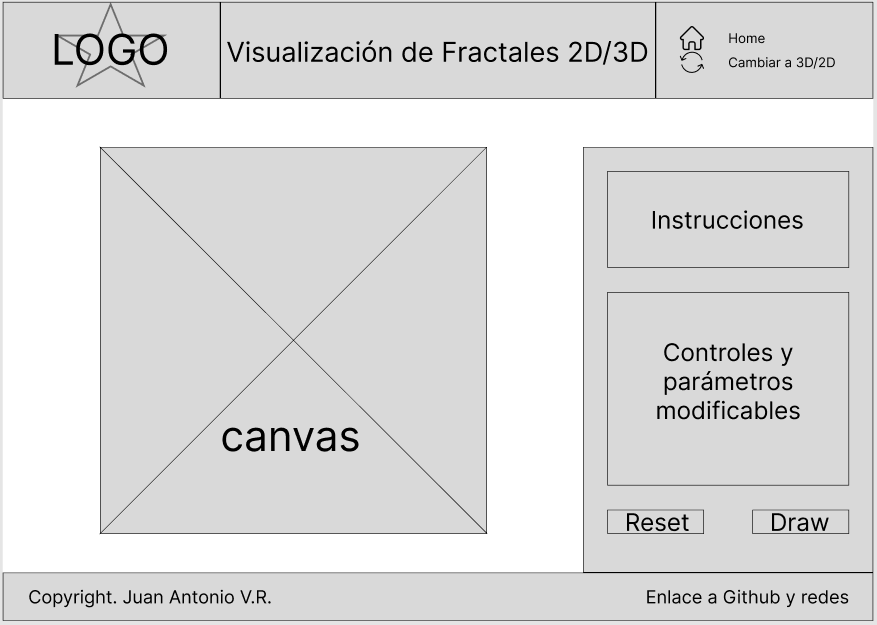
\includegraphics[width=12cm]{img/wireframe-1.png}
    \caption{Wireframe de la pantalla en la que se visualizan fractales}
        \label{fig:wireframe-fractals}
    \end{figure}